\chapter{Experiments}
\label{experiments_chapter}
In this chapter, we will evaluate the performance of the various agents when confronted with different combinations of obstacles. One of the key questions we aim to answer is whether any of the agents are able to successfully learn to play the entire game.

\section{Discounting}
Before diving into the results of the experiments, it is important to note that the discount factor was found to be inconsequential during the experimentation process. Specifically, the agents demonstrated better performance when the discount factor, represented by the variable gamma, was set to 1 (indicating that each step carries equal weight) as opposed to a value less than 1. This outcome is surprising as it would be intuitive to assume that the obstacle in the final step of the episode, which resulted in the agent's death, should be met with a more severe punishment compared to the obstacles encountered earlier in the episode.

\section{Individual Traps}
\begin{figure}[h]
    \centering
    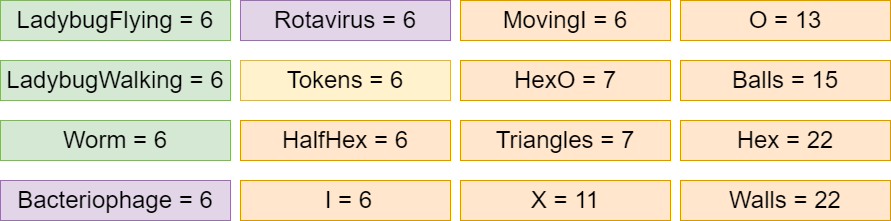
\includegraphics[width=0.4\textwidth]{rot_values}
    \caption{\texttt{rots} value used for each trap type}
    \label{fig:rot_values}
\end{figure}

To start off let us analize each individual type of trap and how the agents perform under the same conditions. For this purpose we have performed experiments for each agent and each trap type with the hope that they can learn to play in such an environment in under 50 games.  In figure \ref{fig:rot_values} we can see the number of rotations used for each individual trap type. The aim was to minimize this number so that the state space itself would be minimized. To calculate how many states there are in an experiment, it is sufficient  to multiply the number of obstacles by the number of possible rotations and distances. However, it is important to mention that throughout this experimentation, \texttt{dists} value was always 1 since all the obstacles were successfully trained by at least one agent with that number of distances.

\begin{figure}[h]
    \centering
    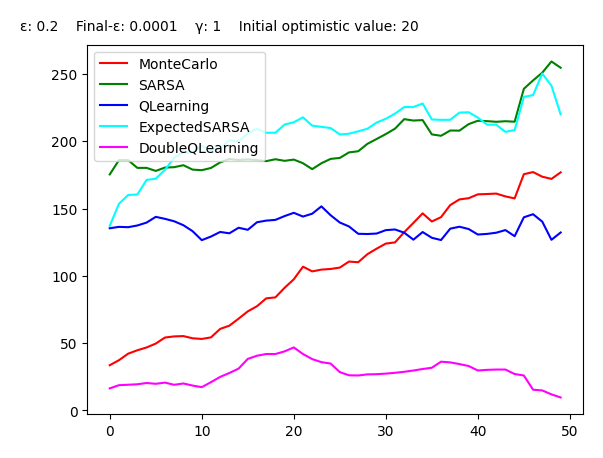
\includegraphics[width=0.6\textwidth]{eps=0.2_initOptVal=20_}
    \caption{Average performance of the agents on individual traps, initOptVal=20}
    \label{fig:avgiop20}
\end{figure}

\begin{figure}[h]
    \centering
    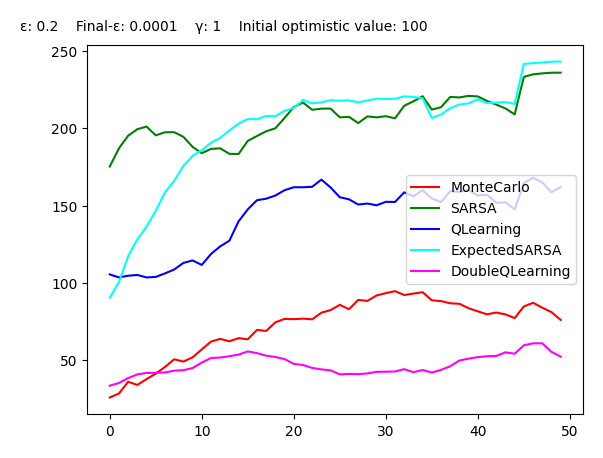
\includegraphics[width=0.6\textwidth]{eps=0.2_initOptVal=100_}
    \caption{Average performance of the agents on individual traps, initOptVal=100}
    \label{fig:avgiop100}
\end{figure}

\begin{figure}[h]
    \centering
    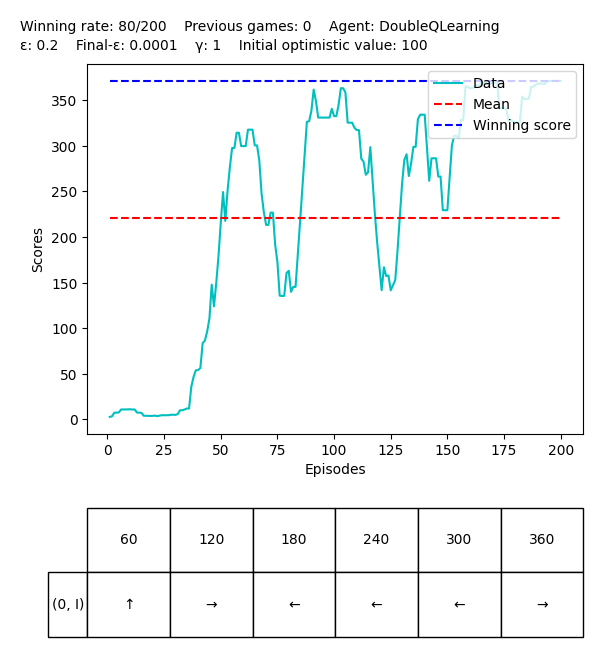
\includegraphics[width=0.8\textwidth]{agent=DoubleQLearning,agentSpecParam=[eps=0.2,epsFinal=0.0001,gam=1,initOptVal=100],level=1,env=[I],shooting=False,dists=1,rots=6_0}
    \caption{Double Q-Learning trained with 200 games on I-type trap}
    \label{fig:dqli}
\end{figure}

In the Figures \ref{fig:avgiop20} and \ref{fig:avgiop100}, we can observe the average performance of each agent in 50 games for individual traps and with different initial optimistic values. Both of these experiments utilized an epsilon value of 0.2. It is evident that the Double Q-Learning agent had the lowest performance among the agents tested in these experiments. However, it is important to note that when trained on a larger number of games, this agent demonstrated improved performance (as seen in Figure \ref{fig:dqli}\footnote{The table on the figure shows the move agent will choose in a certian state. Columns represent rotation value while rows show us which trap and dists value the state has. The value of a particular row and column, then, is an arrow pointing to which direction the agent will move. In case the agent chooses to shoot, a little * will be shown next to the arrow}).

\begin{figure}[h]
    \centering
    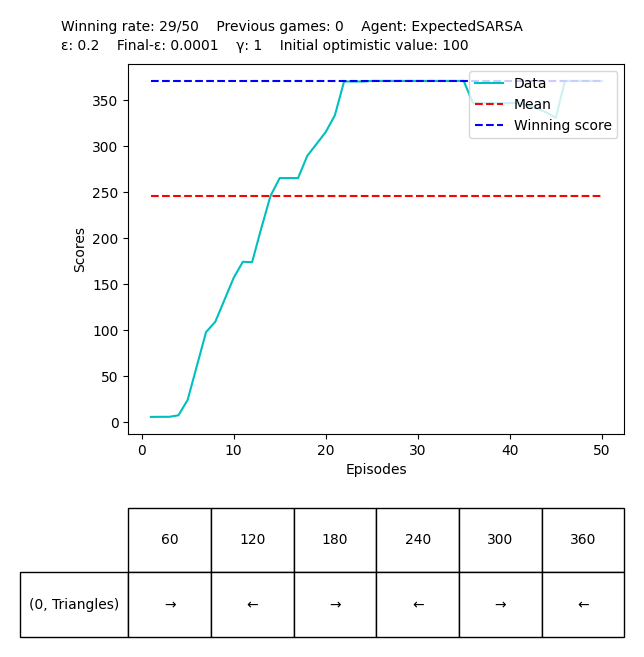
\includegraphics[width=0.7\textwidth]{agent=ExpectedSARSA,agentSpecParam=[eps=0.2,epsFinal=0.0001,gam=1,initOptVal=100],level=1,env=[Triangles],shooting=False,dists=1,rots=6_0
}
    \caption{Triangle-type trap with Expected SARSA algorithm}
    \label{fig:dqli}
\end{figure}

Once peculiar case while training on individual traps is shown in Figure 4. If we look more closely to the policy the agent has chosen, it is visible that instead of aiming to reach a specific rotation value, it decided to rather quickly switch in between two rotations as, in this case, it will always be a safe option. This is indeed the optimal policy for this trap type under six rotations.

\section{Bugs}
In this section, we will analyze how the Bugs environment responded to training with different agents. As seen in Figure \ref{fig:avgbugs}, the SARSA and Expected SARSA agents had the best overall performance in this environment. Interestingly, when shooting was enabled, the policies trained by these algorithms were the same as when shooting was disabled (see Figures \ref{fig:polexps} and \ref{fig:pols}). This result might be counter intuitive since the shooting gains point for the player and, since we did not have energy tokens in this environment, the agent was allowed to shoot indefinitely.

\begin{figure}[h]
    \centering
    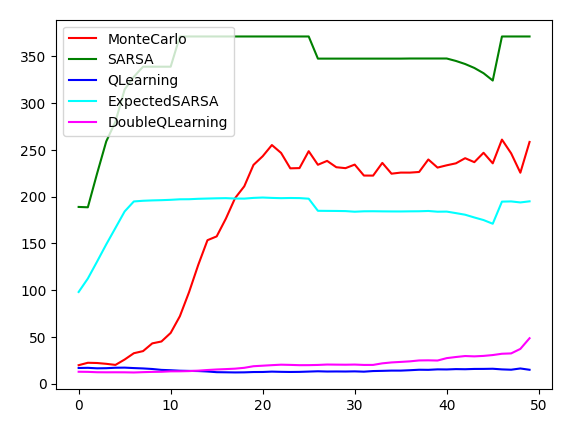
\includegraphics[width=0.6\textwidth]{env=bugs}
    \caption{Average performance of the agents with Bugs environment}
    \label{fig:avgbugs}
\end{figure}

\begin{figure}[h]
    \centering
    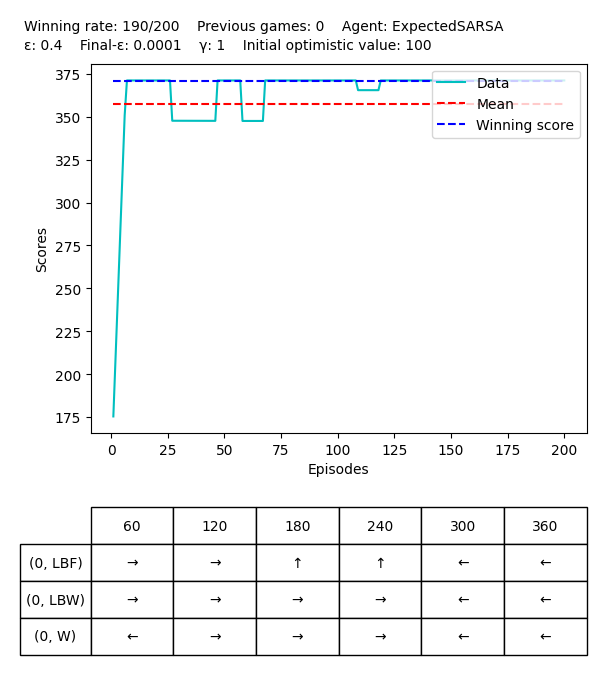
\includegraphics[width=0.7\textwidth]{agent=ExpectedSARSA,agentSpecParam=[eps=0.4,epsFinal=0.0001,gam=1,initOptVal=100],level=1,env=[Bugs],shooting=False,dists=1,rots=6_0}
    \caption{Policy of the Expected SARSA algorithm on the Bugs environment}
    \label{fig:polexps}
\end{figure}

\begin{figure}[h]
    \centering
    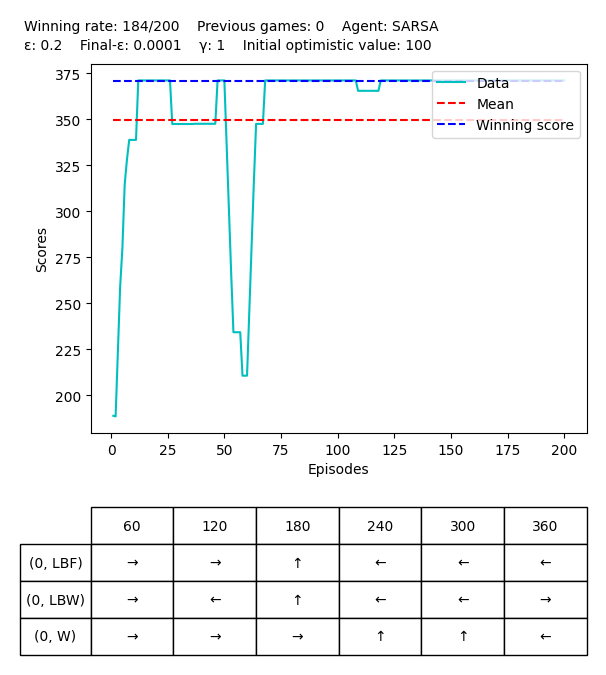
\includegraphics[width=0.7\textwidth]{agent=SARSA,agentSpecParam=[eps=0.2,epsFinal=0.0001,gam=1,initOptVal=100],level=1,env=[Bugs],shooting=True,dists=1,rots=6_0}
    \caption{Policy of the SARSA algorithm on the Bugs environment}
    \label{fig:pols}
\end{figure}

\section{Viruses}

\begin{figure}[h]
    \centering
    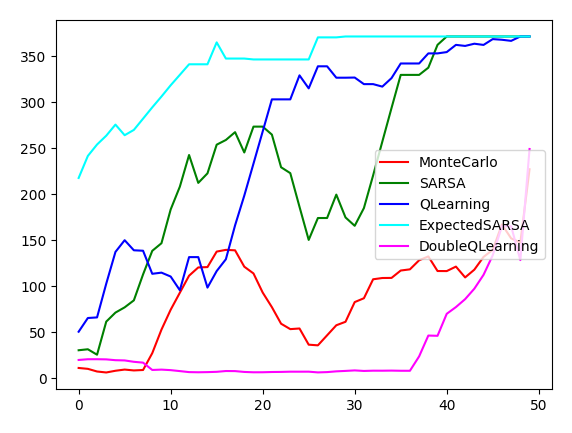
\includegraphics[width=0.6\textwidth]{env=viruses}
    \caption{Average performance of the agents with Viruses environment}
    \label{fig:avgviruses}
\end{figure}

The results of the experiments on the viruses environment indicate that the Expected SARSA and Q-Learning algorithms performed the best. While Q-Learning resulted in the same policy with both shooting enabled and disabled, the Expected SARSA algorithm produced two distinct policies depending on the presence of shooting (see Figures \ref{fig:qvir}, \ref{fig:esvir} and \ref{fig:esvirShooting}). Even when given the option to shoot, the agent preferred to avoid the obstacle instead. A comparison of the performance of all algorithms can be seen in Figure \ref{fig:avgviruses}.


\begin{figure}[h]
    \centering
    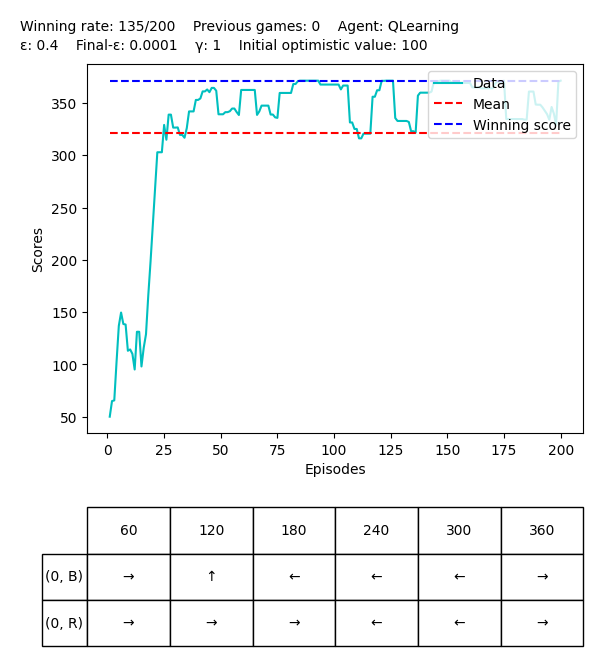
\includegraphics[width=0.7\textwidth]{agent=QLearning,agentSpecParam=[eps=0.4,epsFinal=0.0001,gam=1,initOptVal=100],level=1,env=[Viruses],shooting=True,dists=1,rots=6_0}
    \caption{Policy of the Q-Learning algorithm on the Viruses environment}
    \label{fig:qvir}
\end{figure}

\begin{figure}[h]
    \centering
    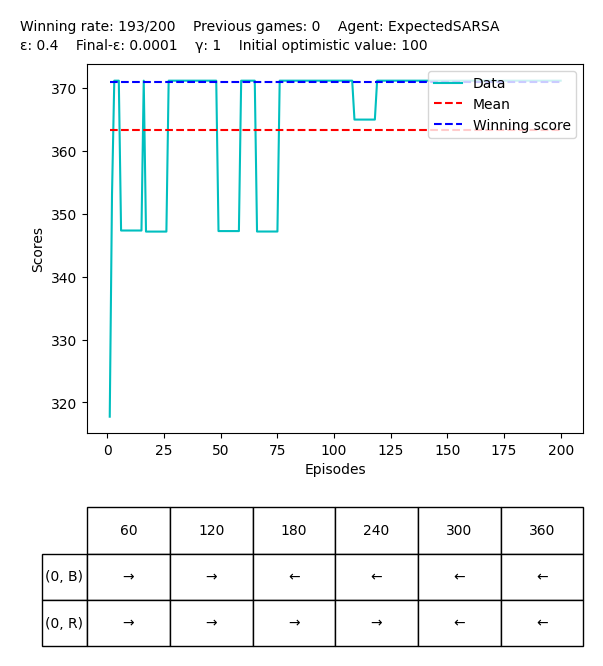
\includegraphics[width=0.7\textwidth]{agent=ExpectedSARSA,agentSpecParam=[eps=0.4,epsFinal=0.0001,gam=1,initOptVal=100],level=1,env=[Viruses],shooting=False,dists=1,rots=6_0}
    \caption{Policy of the Expected SARSA algorithm on the Viruses environment without shooting}
    \label{fig:esvir}
\end{figure}


\begin{figure}[h]
    \centering
    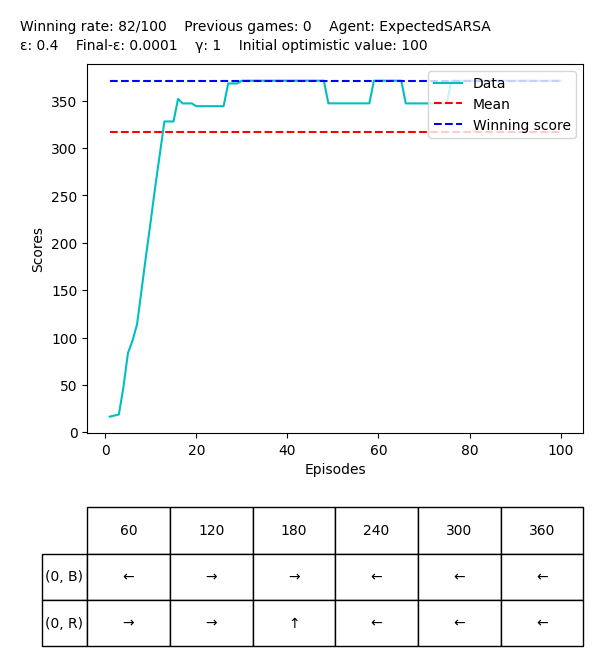
\includegraphics[width=0.7\textwidth]{agent=ExpectedSARSA,agentSpecParam=[eps=0.4,epsFinal=0.0001,gam=1,initOptVal=100],level=1,env=[Viruses],shooting=True,dists=1,rots=6_0}
    \caption{Policy of the Expected SARSA algorithm on the Viruses environment with shooting}
    \label{fig:esvirShooting}
\end{figure}

\section{Tokens}
The results of the experiments conducted in the token environment show that all of the agents had a high success rate in winning the game. Experiments themselves have been performed on 20 games only, since this is the simplest environment we can observe in this project. The comparison of the performance of the different algorithms can be seen in Figure \ref{fig:compTok}.

\begin{figure}[h]
    \centering
    \includegraphics[width=0.7\textwidth]{env=Tokens}
    \caption{Performance comparison of the algorithms on the Token environment}
    \label{fig:compTok}
\end{figure}

\section{Combinations}
In this section, we will examine the performance of the agents in a more complex environment with a larger group of obstacles. This analysis will provide a transition between the simpler experiments and the most challenging task of training on a full game.
\subsection{Traps}
As previously discussed, the algorithms generally demonstrated satisfactory performance when facing individual traps. However, when confronted with all trap types simultaneously, only two algorithms were able to successfully find an optimal policy. It is plausible that with more training or alternate parameters, all algorithms would be capable of reaching an optimal policy. Nonetheless, in these experiments, Monte Carlo and Expected SARSA demonstrated particularly strong performance. For visual representations of the policies developed by these algorithms, see Figures \ref{fig:estraps} and \ref{fig:mctraps}.

\begin{figure}[h]
    \centering
    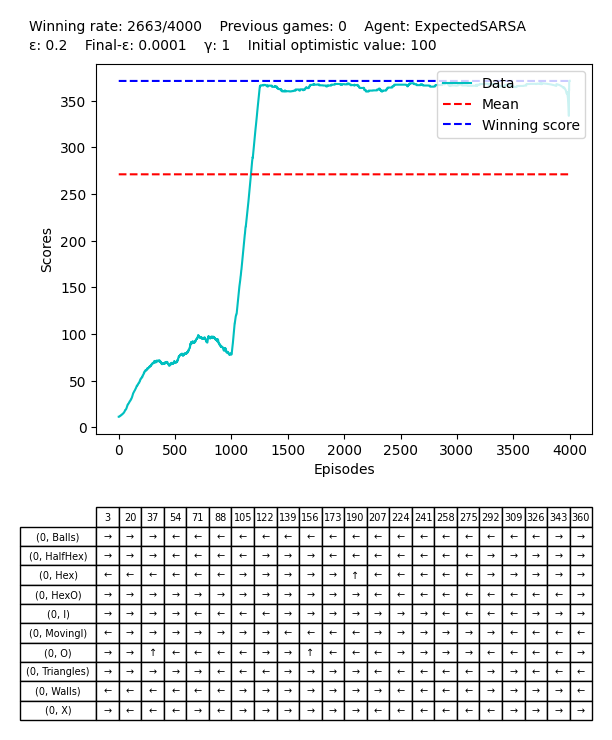
\includegraphics[width=1\textwidth]{agent=ExpectedSARSA,agentSpecParam=[eps=0.2,epsFinal=0.0001,gam=1,initOptVal=100],level=1,env=[Traps],shooting=False,dists=1,rots=22_0}
    \caption{Policy of the Expected SARSA algorithm on the Traps environment}
    \label{fig:estraps}
\end{figure}


\begin{figure}[h]
    \centering
    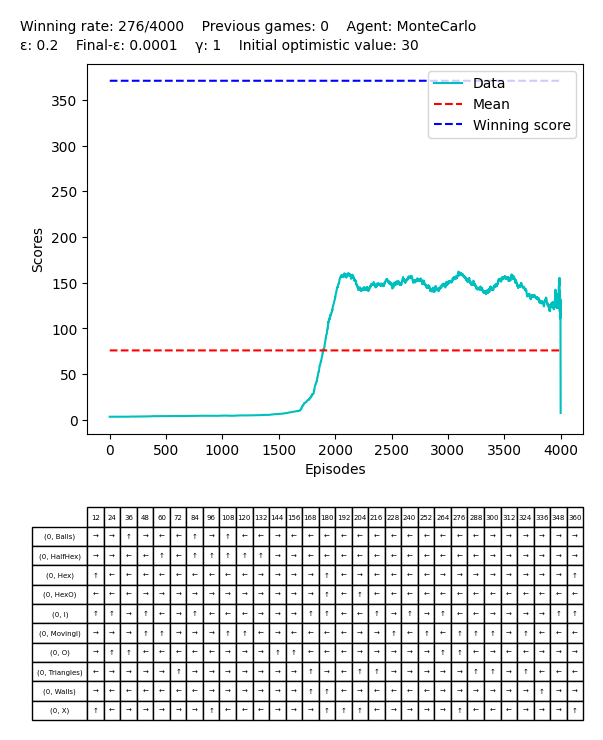
\includegraphics[width=1\textwidth]{agent=MonteCarlo,agentSpecParam=[eps=0.2,epsFinal=0.0001,gam=1,initOptVal=30],level=1,env=[Traps],shooting=False,dists=1,rots=30_0}
    \caption{Policy of the Monte Carlo algorithm on the Traps environment}
    \label{fig:mctraps}
\end{figure}

\subsection{Bugs, Viruses and Tokens}
As previously demonstrated, the Bugs, Viruses, and Tokens agents individually exhibited excellent performance. However, when these agents were combined in our experiments, only the Expected SARSA agent was able to determine an optimal policy for this environment. This policy, depicted in Figure \ref{fig:esbvt}, prioritizes avoiding obstacles rather than shooting them down. The agent appears to prioritize safety over the potential for a higher score by shooting down a bug or virus, as this strategy carries the risk of energy depletion. This preference for a risk-averse approach is consistent with the agent's previous behavior.

\begin{figure}[h]
    \centering
    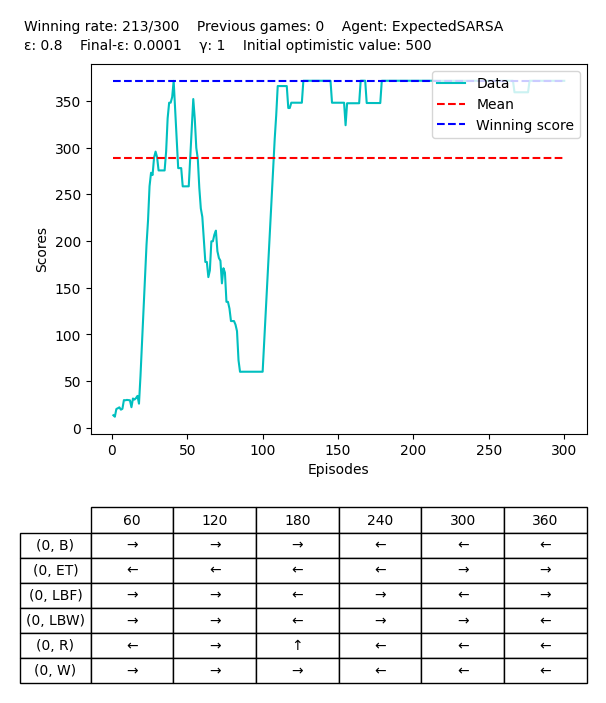
\includegraphics[width=1\textwidth]{agent=ExpectedSARSA,agentSpecParam=[eps=0.8,epsFinal=0.0001,gam=1,initOptVal=500],level=1,env=[Bugs,Tokens,Viruses],shooting=False,dists=1,rots=6_0}
	\caption{Policy of the Expected SARSA algorithm on the Bugs, Viruses and Tokens environment combined}    
    \label{fig:esbvt}
\end{figure}

\section{All obstacles}
Despite its strong performance in previous experiments, the Expected SARSA algorithm did not successfully learn the optimal policy for the whole game during this experimentation. While the policy it developed did win some games, it was not a significant amount. It is possible that different parameters may have resulted in a different outcome, but further research would be necessary to confirm this. The results of this experiment can be seen in Figure \ref{fig:all}.

\begin{figure}[h]
    \centering
    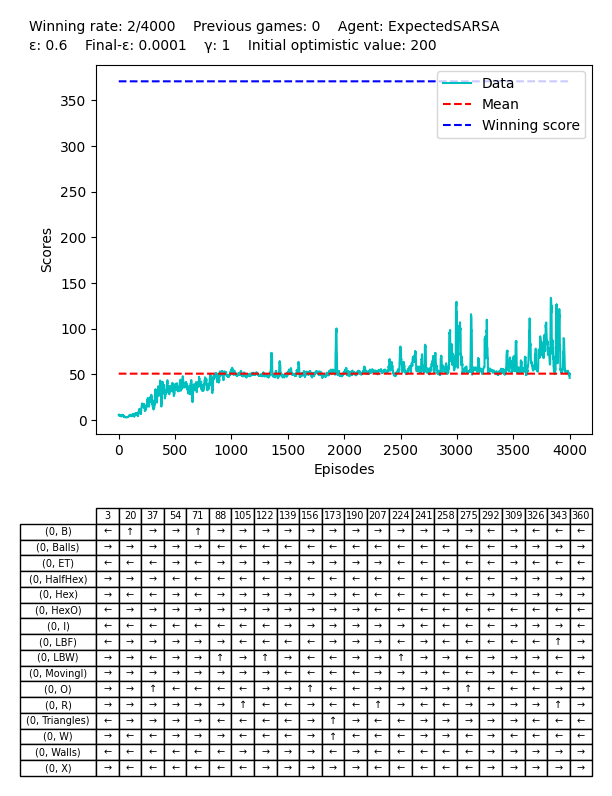
\includegraphics[width=1\textwidth]{agent=ExpectedSARSA,agentSpecParam=[eps=0.6,epsFinal=0.0001,gam=1,initOptVal=200],level=1,env=all,shooting=False,dists=1,rots=22_0}
	\caption{Policy of the Expected SARSA algorithm on the whole game}    
    \label{fig:all}
\end{figure}

